% Jacob Neumann

% DOCUMENT CLASS AND PACKAGE USE
    \documentclass[aspectratio=169, handout]{beamer}

    % Establish the colorlambda boolean, to control whether the lambda is solid color (true), or the same as the picture (false)
    \newif\ifcolorlambda
    \colorlambdafalse % DEFAULT: false

    % Use auxcolor for syntax highlighting
    \newif\ifuseaux
    \useauxfalse % DEFAULT: false

    % Color settings
    \useauxtrue

    \newcommand{\auxColor}{c2ba4c}     % the color of note boxes and stuff
    \newcommand{\presentColor}{0DCAF3} % the primary color of the slide borders
    \newcommand{\bgColor}{e8fbff}      % the color of the background of the slide
    \newcommand{\darkBg}{8b98ad}
    \newcommand{\lambdaColor}{\auxColor}

    \colorlambdatrue

    \usepackage{comment} % comment blocks
    \usepackage{soul} % strikethrough
    \usepackage{listings} % code
    \usepackage{makecell}

    \setbeamertemplate{itemize items}[circle]
    % \setbeameroption{show notes on second screen=right}

    \usepackage{lectureSlides}
    %%%%%%%%%%%%%%%%%%%%%%%%%%%%%%%%%%%%%%%%%| <----- Don't make the title any longer than this
    \title{Lazy Programming} % TODO
    \subtitle{Work harder by working less} % TODO
    \date{25 July 2023} % TODO
    \author{Brandon Wu} % TODO

    \graphicspath{ {./img/} }
    % DONT FORGET TO PUT [fragile] on frames with codeblocks, specs, etc.
        %\begin{frame}[fragile]
        %\begin{codeblock}
        %fun fact 0 = 1
        %  | fact n = n * fact(n-1)
        %\end{codeblock}
        %\end{frame}

    % INCLUDING codefile:
        % 1. In some file under code/NN (where NN is the lecture id num), include:
    %       (* FRAGMENT KK *)
    %           <CONTENT>
    %       (* END KK *)

    %    Remember to not put anything on the same line as the FRAGMENT or END comment, as that won't be included. KK here is some (not-zero-padded) integer. Note that you MUST have fragments 0,1,...,KK-1 defined in this manner in order for fragment KK to be properly extracted.
        %  2. On the slide where you want code fragment K
                % \smlFrag[color]{KK}
        %     where 'color' is some color string (defaults to 'white'. Don't use presentColor.
    %  3. If you want to offset the line numbers (e.g. have them start at line 5 instead of 1), use
                % \smlFragOffset[color]{KK}{5}

\begin{document}

% Make it so ./mkWeb works correctly
\ifweb
    \renewcommand{\pause}{}
\fi

\setbeamertemplate{itemize items}[circle]

% SOLID COLOR TITLE (see SETTINGS.sty)
{
\begin{frame}[plain]
    \colorlambdatrue
    \titlepage
\end{frame}
}

\menti{6919 7141}

\begin{frame}[fragile]
  \frametitle{Lesson Plan}

  \tableofcontents
\end{frame}

\sectionSlide{1}{Lazy Evaluation}

\begin{frame}[fragile]
  \frametitle{A First For Everything}

  Consider the following simple SML function:
  \begin{codeblock}
    fun fst (x, y) = x
  \end{codeblock}

  \pause
  \vspace{\fill}

  This is usually a pretty standard function to have around, for instance
  if you want to get out the first component of a tuple without pattern
  matching (for instance, if you're doing a pipe chain).

  \pause
  \vspace{\fill}

  \textbf{Question:} What is the behavior of the expression \code{fst (1, 1 div 0)}?
\end{frame}

\begin{frame}[fragile]
  \frametitle{Waste Not}

  \textbf{Answer:} It raises \code{Div}.

  \pause
  \vspace{\fill}

  Recall that this is due to the fact that SML is a \term{eagerly evaluated} language,
  and the arguments to functions are always evaluated to values, if possible, before
  stepping into the body of the function.

  \pause
  \vspace{\fill}

  But this is kind of silly, right? We wanted the first component of this tuple. It
  shouldn't matter whether the second component raises an exception -- our code was
  only concerned with the first part.

  \pause
  \vspace{\fill}

  The same thing would happen even if the second component didn't loop forever or
  raise an exception, but instead took a very long time! For instance,
  \code{fst (1, horribleComputation 2 4)} would similarly take a long time.
  \footnote{By my reckoning, 3 years.}
\end{frame}

\begin{frame}[fragile]
  \frametitle{Want Not}

  Or, if we performed \code{map f L} on a list, but only used the first few elements.

  \pause
  \vspace{\fill}

  This doesn't stop the fact that the \code{map} function always fully commits,
  and applies the function \code{f} to \textit{each element} of the input list.
  It doesn't know anything about whether the result will be used, it's simply
  following the rules of eager evaluation.

  \pause
  \vspace{\fill}

  The theme is the same -- we want not to do work if we can avoid it. We want
  to only have to do a computation if we \textit{have} to. In other words, we
  want to be \term{lazy}.
\end{frame}

\begin{frame}[fragile]
  \frametitle{Lazy Evaluation}

  \defBox{}{\term{Lazy evaluation} is a schema of evaluation opposite to
  that of eager evaluation. In lazy evaluation, instead of evaluating expressions
  at val bindings and function invocations, we only evaluate expressions when their
  value is \textit{needed}.
  }

  \pause
  \vspace{\fill}

  So for instance, the following:
  \begin{codeblock}
    val L = [999, 998, 997, 996, 995]
    val res =
      List.foldl (fn (x, acc) => fact (fact (x * acc))) 1 L
  \end{codeblock}
  \pause
  would run almost instantly, if SML were to be a lazy language. This is because
  under eager evaluation, we would instantly evaluate the right-hand side of
  \code{res}, which takes approximately between ludicrously long and forever.
\end{frame}

\begin{frame}[fragile]
  \frametitle{Lazy Variables}

  Under lazy evaluation, we have to do no such thing, however! We can instantly
  bind \code{res}, by binding it to the verbatim expression of its RHS.

  \pause
  \vspace{\fill}

  A way to think of the conceptual difference between lazy and eager evaluation
  is that in an eager language, variables can only be bound to values, which
  cannot further be simplified. In a lazy language, \textbf{variables are bound to
  expressions}, which are simplified upon \term{forcing} the expression.

  \pause
  \vspace{\fill}

  For instance, if we tried to evaluate this code in the context of the previous
  slide:
  \begin{codeblock}
    case res of
      0 => 1
    | _ => 2
  \end{codeblock}
  then, we would be forced to evaluate the expression that \code{res} is bound
  to, because we want to see what value it has.
\end{frame}

\begin{frame}[fragile]
  \frametitle{The Problems with Laziness}

  Laziness seems great. You only ever need to pay for what you need --
  wasted computation is impossible. There's some technical details around
  implementation that warrant a little more special consideration, but otherwise
  it seems like a good deal.

  \pause
  \vspace{\fill}

  The problem with laziness comes with a \textbf{lack of predictability}.
\end{frame}

\begin{frame}[fragile]
  \frametitle{A Lazy Exchange}

  Consider the following scenario in a lazy programming language. You have
  implemented an API which returns to a user an \code{int list}.

  \pause
  \vspace{\fill}

  A consumer reads your documentation, believes it's just what they need for
  their project, so they pull down your code and invoke your function and
  bind the result to a variable. They then proceed on their merry way.

  \pause
  \vspace{\fill}

  120 production hours later, their web server crashes due to an unexpected
  error.

  \pause
  \vspace{\fill}

  The list that you handed them was \code{[raise Div, raise Div, raise Div]}.
\end{frame}

\begin{frame}[fragile]
  \frametitle{A Lazy Exchange}

  This might seem like a ridiculous example, but the point is that in a
  lazy language, all data exchange can be completely arbitrary computation!

  \pause
  \vspace{\fill}

  In an eager language, if you are able to receive an output and bind it
  to a variable, you are guaranteed that you are holding real data. In the
  case of the poor consumer, they were handed a list of three ticking time
  bombs. These time bombs were only revealed 120 hours later, when the elements
  of the list were presumably actually accessed and forced.

  \pause
  \vspace{\fill}

  This can make nightmarish bugs arise, because ultimately
  \textbf{computation is unpredictable}. You have no idea when a value will be
  forced, because it could happen now or many hours later.
\end{frame}

\begin{frame}[fragile]
  \frametitle{Lazy Performance}

  It doesn't even need to be a list of \code{raise Div}, this also has
  implications for determining performance. You could be handed a list
  of expressions, all of which take quite a while to evaluate. Now, in
  applications where you can't necessarily afford to wait around for
  several seconds, you need to be careful any time you case on an expression.

  \pause
  \vspace{\fill}

  You also ultimately get that functions like \code{map f} are constant time,
  and it's only when they are forced that a linear cost in \code{f} comes
  about. This makes it very difficult to give performance a rigorous treatment.
  \footnote{Lazy languages also don't have sum types. This is of absolutely no
  relevance to anyone in this course, but I'm obliged to say it.}
\end{frame}

\begin{frame}[fragile]
  \frametitle{What's The Point?}

  Well, that's a lot of negatives. SML is an eager language anyways, so what's
  the big whoop? Why are we talking about lazy evaluation?

  \pause
  \vspace{\fill}

  What does binding a variable to something which encodes a \textit{computation}
  without actually evaluating it sound like?

  \pause
  \vspace{\fill}

  Suppose we wanted to mimic something which in a lazy language looked like
  this:
  \begin{codeblock}
    val res = map f L
  \end{codeblock}

  \pause
  \vspace{\fill}

  Recall the idea of a lambda function as a \textit{suspension}:
  \begin{codeblock}
    val res = `fn () =>` map f L
  \end{codeblock}
  %'

  \pause
  \vspace{\fill}

  It turns out, we can mimic laziness in an eager language, just by using
  lambdas.
\end{frame}

\begin{frame}[fragile]
  \frametitle{Thunks}

  \defBox{}{A \term{thunk}\footnote{Yes, this is a technical term.} is a value of type \code{unit -> t}, for some
  type \code{t}, also called a \term{suspension}.}

  \pause
  \vspace{\fill}

  For any expression \code{e}, we can turn it into a thunk by simply encasing
  it within a lambda expression. Recall that lambda expressions \textit{freeze}
  the contents of their bodies, meaning that no evaluation happens until the
  lambda is given an argument!

  \pause
  \vspace{\fill}

  \keyBox{\, Lambdas \textit{suspend} the contents of their bodies until the function
  is actually called.}

  \pause
  \vspace{\fill}

  By convention, that lambda usually just takes in a unit argument,
  since we don't really care about doing anything with its input, we just
  want to prevent the computation.
\end{frame}

\begin{frame}[fragile]
  \frametitle{The Benefits of Laziness}

  Laziness has a lot of problems, but that is only when it is \textit{on by default}!

  \pause
  \vspace{\fill}

  Something we will see, in this lecture and the next, is that language features are
  generally better when they are \textit{opt-in}. Programmers should have full
  control over what behavior they want, and shouldn't be forced into something
  contentious.

  \pause
  \vspace{\fill}

  The great strength of an eager language is that we can \textit{simulate laziness},
  by putting computations into a lambda, which is to be evaluated at a later time.

  \pause
  \vspace{\fill}

  This way, we can take advantage of the benefits of laziness, such as not needing
  to compute things until we need to and not wasting computation, without
  suffering the disaster of having it on all the time!
\end{frame}

\sectionSlide{2}{A Lazy Structure}

\begin{frame}[fragile]
  \frametitle{A Lazy Type}

  In fact, this idea is so powerful that it will warrant its own module, and type.

  \pause
  \vspace{\fill}

  \begin{codeblock}
    signature LAZY =
      sig
        (* The type of lazy suspensions of type 'a. These are
           computations which may return an 'a.
         *)
        type 'a t

        val lazy : (unit -> 'a) -> 'a t
        val force : 'a t -> 'a
      end
  \end{codeblock}
\end{frame}

\begin{frame}[fragile]
  \frametitle{A Lazy Module}

  \tgs

  Here, the type of \code{Lazy.t} is kept abstract, to signal a type-level
  distinction between this idea of suspended computations versus actual values.

  \pause
  \vspace{\fill}

  \begin{codeblock}
    structure Lazy :> LAZY =
      struct
        type 'a t = unit -> 'a

        fun lazy f  = f
        fun force f = f ()
      end
  \end{codeblock}

  In reality, the type of \code{'a t} is exactly equivalent to \code{unit -> 'a},
  so the \code{lazy} function doesn't "really" do anything.

  \pause
  \vspace{\fill}

  But to the user of the library, they don't know that. The point is that this
  kind of conceptual separation is useful, because it helps us segment our
  thinking.
\end{frame}

\begin{frame}[fragile]
  \frametitle{A Lazy Example}

  So for instance, in the following code:
  \begin{codeblock}
    val L = List.tabulate (100, fn i => lazy (fn () => i * i))
  \end{codeblock}
  the produced list \code{L} is a \code{int Lazy.t list}, where the $i$th
  entry is a \textit{suspension} of the $i$th square number, that can be forced at a
  later time. This way, we avoid computing all of the squares up front, in case
  that we don't actually need all of them.

  \pause
  \vspace{\fill}

  This example is reasonably contrived, but lazy values can be very useful for
  certain kinds of computations that may be needed later but are costly to do
  all at once, such as when reading from files.

  \pause
  \vspace{\fill}

  Usually, lazy values are also \term{memoized}, which means forcing them only
  ever computes the expression once, and then saves the result for future forces.
  This implementation omits that, but this is the general practice.
\end{frame}

\quizBreak{\textlangle obfuscated\textrangle}

\sectionSlide{3}{Infinite Data Structures}

\begin{frame}[fragile]
  \frametitle{An Industrial Example}

  Suppose that the CEO of your company comes into the room, and tells you she
  wants all the integers.

  \pause
  \vspace{\fill}

  You tell her, boss, I don't know if you know this, but the integers are infinite.

  \pause
  \vspace{\fill}

  She says actually yes, she was perfectly aware of that, and was she going crazy
  or did she hear something which sounded like talking back to her.

  \pause
  \vspace{\fill}

  You tell her you'll try your best.
\end{frame}

\begin{frame}[fragile]
  \frametitle{Don't Do This At Home}

  The situation is not dissimilar to the following:

  \pause
  \vspace{\fill}

  \begin{center}
  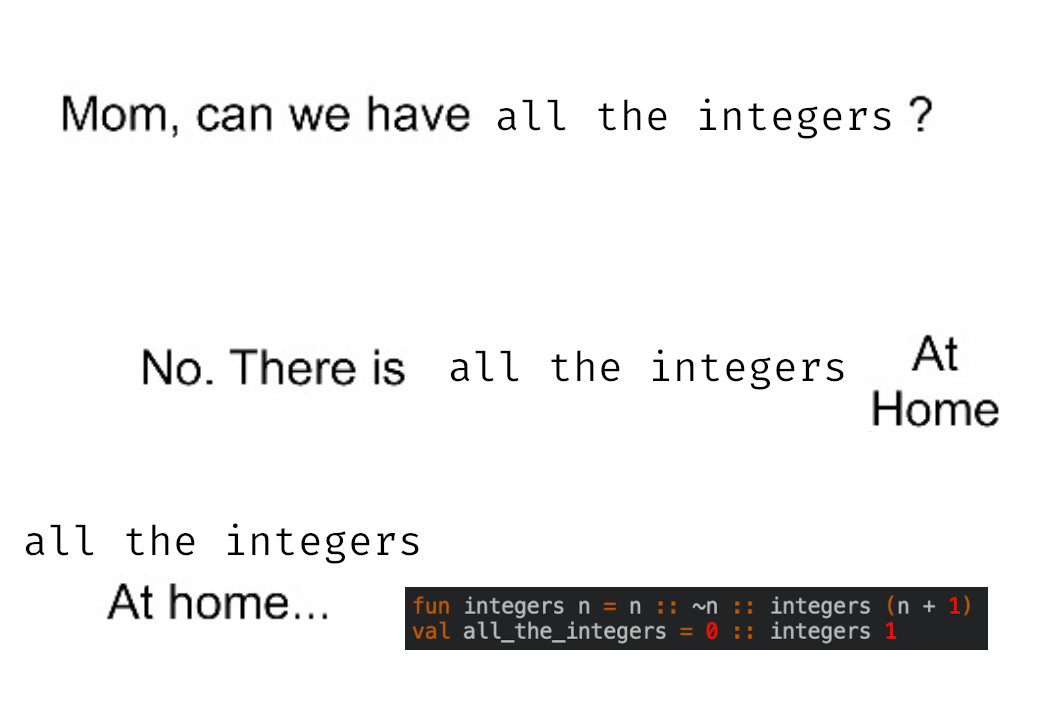
\includegraphics[scale=0.85]{all_the_integers.png}
  \end{center}

  \pause
  \vspace{\fill}

  The key issue at hand here is that the integers are infinite, and thus
  computing \code{all_the_integers} loops forever.
\end{frame}

\begin{frame}[fragile]
  \frametitle{I Reject Your Reality}

  The integers are nicely mathematically defined, however. It's a real shame
  that we should be limited by silly concerns like "lack of infinite amounts
  of space", and thus be unable to store all of the integers.

  \pause
  \vspace{\fill}

  It's impossible to have infinitely many processors too, though.\footnote{\textit{citation needed}}
  We don't usually let silly things like physical impossibility get in our way --
  can we figure out something here too?
\end{frame}

\begin{frame}[fragile]
  \frametitle{Infinite Data Structures}

  This leads us into an idea called \term{infinite data structures}.

  \vspace{\fill}

  \defBox{}{An \term{infinite data structure} is a kind of data structure
  that may store infinitely many entries, without looping forever.}

  \pause
  \vspace{\fill}

  The memory concern is still a legitimate one, though. We can't possibly store
  an infinite number of numbers at once, so what can we do?

  \pause
  \vspace{\fill}

  The key to encoding infinite data structures will be in using \term{laziness},
  to compute entries only as we need them.
\end{frame}

\begin{frame}[fragile]
  \frametitle{Lazy Lists}

  \rprs

  Our first data structure will be the \term{lazy list}. Recall that
  we could define our own type of lists via the following:
  \begin{codeblock}
    datatype 'a list' = Nil | Cons of 'a * 'a list'
  \end{codeblock}
  which would be totally equivalent to our native type of \code{'a list}.

  \pause
  \vspace{\fill}

  We can define lazy lists as follows:
  \begin{codeblock}
    datatype 'a llist = Nil | Cons of 'a * `(unit ->` 'a llist`)`
  \end{codeblock}
  %'

  \pause
  \vspace{\fill}

  Whereas a list is either empty or a value and another list, a lazy list
  is either empty or a value and a \textit{suspension} of another lazy list.
\end{frame}

\begin{frame}[fragile]
  \frametitle{Lazy Lists}

  What does that mean? It means that when forming a value of type \code{'a llist},
  we don't ever need to go and come up with the lazy list that comes afterwards --
  we just need to provide a lambda that computes it.

  \pause
  \vspace{\fill}

  By our analogy from CPS lecture, we just provide \textbf{instructions} that
  tell us how to make the rest of the lazy list.

  \pause
  \vspace{\fill}

  Here are some examples of values of type \code{t llist}:
  \pause
  \begin{itemize}
    \item \code{Nil : 'a llist} \pause
    \item \code{Cons (1, fn () => Nil) : int llist} \pause
    \item \code{Cons (1, fn () => Cons (2, fn () => Nil)) : int llist} \pause
    \item \code{Cons (1, fn () => loop ()) : int llist}
  \end{itemize}

  \pause
  \vspace{\fill}

  Notably, the last value is indeed a value, but trying to get the second
  element of the list will cause an infinite loop.\footnote{That's how it is, sometimes.}
\end{frame}

\begin{frame}[fragile]
  \frametitle{Constructing Lazy Lists}

  \rprs

  Part of the point of lazy lists is that usually, instead of writing them down
  in a finite amount of space, we will construct lazy lists via recursive functions.

  \pause
  \vspace{\fill}

  Let's see how we might define the natural numbers using lazy lists:
  \begin{codeblock}
    fun natsFrom n = Cons (n, fn () => natsFrom (n + 1))
    val nats = natsFrom 0
  \end{codeblock}

  \pause
  \vspace{\fill}

  Here, we define first a helper function \code{natsFrom}, which defines a
  lazy list of all the natural numbers, from some starting point. Then, we just
  start at 0.

  \pause
  \vspace{\fill}

  Note that because the recursive call to \code{natsFrom} is within a thunk,
  there is no looping forever here! For that same reason, we don't need a base
  case, either.
\end{frame}

\begin{frame}[fragile]
  \frametitle{Constructing Arbitrary Lazy Lists}

  Suppose that we were interested in tabulating a lazy list from an
  arbitrary function. We might define a function \code{tabulate} with the
  following specification:

  \pause
  \spec
    {lazyTabulate}
    {(int -> 'a) -> 'a llist}
    {\code{true}}
    {\code{lazyTabulate f} evaluates to the lazy list where the \code{i}th
    element is \code{f i}}

  \pause
  \vspace{\fill}

  \begin{codeblock}
    fun lazyTabulateFrom f i =
      Cons (f i, fn () => lazyTabulateFrom f (i + 1))
    fun lazyTabulate f = lazyTabulateFrom f 0
  \end{codeblock}
\end{frame}

\begin{frame}[fragile]
  \frametitle{Constructing Arbitrary Lazy Lists}

  Let's try it on a specific use case.

  \pause
  \vspace{\fill}

  \begin{codeblock}
    val lazy_list = lazyTabulate (fn i => 1024 div i)
  \end{codeblock}

  \pause
  \vspace{\fill}

  This lazy list purportedly contains all the results of dividing
  1024 by the natural numbers.

  \vspace{\fill}

  Unfortunately, there is one thing working against us, here, which is
  that 0 is a natural number!

  \pause
  \vspace{\fill}

  Are we OK, though, since this is a lazy list? It turns out no, because
  while our list is lazy, attempting to bind \code{lazy_list} immediately
  raises \code{Div}.
\end{frame}

\begin{frame}[fragile]
  \frametitle{Thresholds of Laziness}

  It turns out that our notion of lazy lists is indeed lazy, but not
  lazy enough.

  \pause
  \vspace{\fill}

  Even if there is an element in the lazy list that should raise \code{Div}
  upon being forced, merely constructing the value of \code{lazy_list}
  never expresses intent to force that element!

  \pause
  \vspace{\fill}

  Or, put another way, we \textbf{never once} explicitly said
  we wanted to look at the elements of the lazy list, so why should constructing
  the lazy list raise an exception on us?

  \pause
  \vspace{\fill}

  In the next section, we'll see an improvement on lazy lists we call \term{streams},
  which will help with this issue.
\end{frame}

\sectionSlide{4}{Maximal Laziness and Streams}

\begin{frame}[fragile]
  \frametitle{Maximal Laziness}

  To solve our problem, we need a new kind of data structure.

  \pause
  \vspace{\fill}

  \defBox{}{A \term{maximally lazy} data structure is one which does not compute
  any element until it is absolutely needed.\footnote{There will be a formal
  definition of this on the homework which is slightly different, but this definition
  will suffice to get us through the intuition.}}

  \pause
  \vspace{\fill}

  We will develop a new type of lazy list called a \code{stream}, which side steps
  these issues by being maximally lazy. We can define a stream via two mutually
  recursive data types:

  \begin{codeblock}
    datatype 'a stream = Stream of (unit -> 'a front)
    and 'a front = Nil | Cons of 'a * 'a stream
  \end{codeblock}

  \pause
  \vspace{\fill}

  Note that we use the \code{and} keyword here, which allows two mutually recursive
  types to see each other, irrespective of the order in which both are declared.
\end{frame}

\begin{frame}[fragile]
  \frametitle{Streams and Fronts}

  \tgs

  Conceptually, what's the idea behind a stream and a front?

  \pause
  \vspace{\fill}

  \keyBox{}{\textbf{A stream is a delayed front.}}
  \pause
  \keyBox{}{\textbf{A front is an exposed stream.}}

  \pause
  \vspace{\fill}

  A stream is opaque -- the only thing you can do with a stream
  is force it. This solves our issue from lazy lists, as instead of making lazy
  lists (which have the first element forced by default), we make streams.

  \pause
  \vspace{\fill}

  A front is a stream which the user has \textbf{expressed intent to force}. The
  only way to obtain a front is to deliberately try to force a stream. The front
  has the actual pattern-matching data associated with it though, which may
  produce another stream.
\end{frame}

\begin{frame}[fragile]
  \frametitle{Literally \code{STREAM}ing}

  We will have another structure for dealing with streams. This one will similarly
  have another an abstract type hiding the inner implementation.

  \pause
  \vspace{\fill}

  \begin{codeblock}
    signature STREAM =
      sig
        type 'a stream
        datatype 'a front = Empty | Cons of 'a * 'a stream

        (* more... *)
      end
  \end{codeblock}

  \pause
  \vspace{\fill}

  These types are implemented exactly the same as the \code{'a stream} and
  \code{'a front} we saw earlier! We just hide the definition of \code{'a stream}
  so it simply operates as an abstract idea of some suspended list, which may
  be forced to look at its contents as a \code{'a front}.
\end{frame}

\begin{frame}[fragile]
  \frametitle{A \code{Stream} Structure}

  We will now look at some of the residents of the \code{Stream} structure.
  There are more functions, which are available at the
  {\color{blue} \href{http://www.cs.cmu.edu/~15150/resources/libraries/stream.pdf}{online 150 documentation}},
  but we will not get to all of them.

  \pause
  \vspace{\fill}

  For the rest of the lecture, assume we are working within the \code{Stream}
  structure, defined as:

  \begin{codeblock}
    structure Stream :> STREAM =
      struct
        datatype 'a stream = Stream of (unit -> 'a front)
        and 'a front = Empty | Cons of 'a * 'a stream

        (* ... *)
      end
  \end{codeblock}
\end{frame}

\begin{frame}[fragile]
  \frametitle{\code{delay} and \code{expose}}

  The most essential functions to working with streams are \code{delay}
  and \code{expose}, which mediate the relationship between \code{stream}s and
  \code{front}s.

  \pause
  \vspace{\fill}

  \spec
    {delay}
    {(unit -> 'a front) -> 'a stream}
    {\code{true}}
    {\code{delay f} creates the stream associated with the thunk \code{f}.}

  \pause
  \vspace{\fill}

  \spec
    {expose}
    {'a stream -> 'a front}
    {\code{true}}
    {\code{expose S} forces the stream \code{S}, revealing the resulting front.
    This does not necessarily need to produce a value!}
\end{frame}

\begin{frame}[fragile]
  \frametitle{\code{delay} and \code{expose}}

  We can implement them as so.

  \pause
  \vspace{\fill}

  \begin{codeblock}
    fun delay f = Stream f
  \end{codeblock}

  \vspace{\fill}

  \begin{codeblock}
    fun expose (Stream f) = f ()
  \end{codeblock}

  \pause
  \vspace{\fill}

  We will use these two functions as helpers when we write functions that operate
  on streams.

  \pause
  \vspace{\fill}

  Since our \code{'a stream} type is abstract, we have to provide these helpers, as
  users of the structure cannot apply the \code{Stream} constructor directly, or
  force the thunk. It ends up that using the \code{delay} and \code{expose} functions
  will make it very explicit when we are doing work and when we are suspending.
\end{frame}

\begin{frame}[fragile]
  \frametitle{A Stream of Naturals}

  Let's try to do the natural numbers again, but this time with streams.

  \pause
  \vspace{\fill}

  We will usually construct streams via \term{mutual recursion}, which is
  functions which are allowed to call each other. This is again achieved
  with the \code{and} keyword.

  \pause
  \vspace{\fill}

  \begin{codeblock}
    fun nats  (i : int) : int stream = delay (fn () => nats' i)
    and nats' (i : int) : int front  = Cons (i, nats (i + 1))
  \end{codeblock}

  \pause
  \vspace{\fill}

  Alternatively, we could have implemented it with a single function:
  \begin{codeblock}
    fun nats i = delay (fn () => Cons (i, nats (i + 1)))
  \end{codeblock}
  but it's generally cleaner to separate into two functions, one of which
  produces a stream, and one of which produces a front. Remember, types
  guide structure.
\end{frame}

\begin{frame}[fragile]
  \frametitle{Constructing Arbitrary Streams}

  We can do \code{tabulate} again, too, but for streams!

  \pause
  \vspace{\fill}

  \begin{codeblock}
    fun tabulateHelp  f i = delay (fn () => tabulateHelp' f i)
    and tabulateHelp' f i = Cons (f i, tabulateHelp f (i + 1))

    fun tabulate f = tabulateHelp f 0
  \end{codeblock}

  \pause
  \vspace{\fill}

  \customBox{Check your understanding}{\, Make sure you understand why
  this version of \code{tabulate} is more lazy than \code{lazyTabulate}.
  What does \code{tabulate f} return, versus \code{lazyTabulate}?}
\end{frame}

\begin{frame}[fragile]
  \frametitle{Mapping Streams}

  Like most data structures, we can write a \code{map} function on streams.

  \pause
  \vspace{\fill}

  \spec
    {map}
    {('a -> 'b) -> 'a stream -> 'b stream}
    {\code{f} is total}
    {\code{map f S} evaluates to the same stream as \code{S}, but with
    \code{f} applied to each element of the stream}

  \pause
  \vspace{\fill}

  \spec
    {map'}
    {('a -> 'b) -> 'a front -> 'b front}
    {\code{f} is total}
    {\code{map' f F} evaluates to the same front as \code{F}, but with
    \code{f} applied to each element of the front}

  \pause
  \vspace{\fill}

  Here, we again define two functions, one for streams and one
  for fronts. Since \code{map} operates on a given stream, the
  corresponding \code{map'} also takes in a front.
\end{frame}

\begin{frame}[fragile]
  \frametitle{Mapping Streams}

  \begin{codeblock}
    fun map  f S = delay (fn () => map' f (expose S))
    and map' f Nil = Nil
      | map' f (Cons (x, s)) = Cons (f x, map f s)
  \end{codeblock}

  \pause
  \vspace{\fill}

  In this case, our mutual recursive usage of these two functions reflects a
  difference in intention between the two functions. When "deconstructing" a
  stream, the function which produces a stream simply sets up the second
  function -- the second function is the only one which actually has license
  to look at the stream's elements.
\end{frame}

\begin{frame}[fragile]
  \frametitle{A Lack of Maximal Laziness}

  The following implementation would fail to be maximally lazy, however.

  \pause
  \vspace{\fill}

  \begin{codeblock}
    fun map f s =
      case expose s of
        Nil => delay (fn () => Nil)
      | Cons (x, s') => delay (fn () => Cons (f x, map f s'))
  \end{codeblock}

  \pause
  \vspace{\fill}

  The process of mapping this stream exposes the input stream, without any
  outside prompting to force the resulting stream! We want to be
  able to map it in a way that we never need to expose any elements, until
  we must.

  \pause
  \vspace{\fill}

  In general, it's only safe to execute operations on a stream so long as
  they are locked behind a call to \code{delay}, so that it only occurs
  once the stream is exposed.
\end{frame}

\begin{frame}[fragile]
  \frametitle{A Lesson in Productivity}

  Recall that exposing a stream means to express intent to look at its elements,
  and will cause the computation of the next element, if any.

  \pause
  \vspace{\fill}

  This is dangerous, because that computation might do anything from raise an
  exception, to loop forever, to take 2 months to run. Exposing a stream is a
  risky endeavour!

  \pause
  \vspace{\fill}

  Generally, we like to work with streams that have well-defined contents, such
  that exposing will always eventually give us another element. We call those
  streams \term{productive}.

  \pause
  \vspace{\fill}

  \defBox{}{ A \term{productive} stream \code{S} is one such that
  \code{Stream.expose S} always terminates with \code{Empty} or
  \code{Cons (x, S')}, where \code{S'} is again productive.}
\end{frame}


\begin{frame}[fragile]
  \frametitle{A Lesson in Productivity}

  Generally, we like working with productive streams. Thus, we need to be
  careful when using functions like \code{map}, which could turn a productive
  stream into a no-longer productive stream.

  \pause
  \vspace{\fill}

  Productivity will also help us describe the specification of more stream
  functions.

  \pause
  \vspace{\fill}

  \spec
    {append}
    {'a stream * 'a stream -> 'a stream}
    {\code{S1} and \code{S2} are productive}
    {\code{append (S1, S2)} is productive}

  \pause
  \vspace{\fill}

  \spec
    {append'}
    {'a front * 'a stream -> 'a front}
    {\code{S2} is productive and \code{F} is \code{Empty} or \code{Cons} of a productive stream}
    {\code{append' (F, S2)} is productive}
\end{frame}

\begin{frame}[fragile]
  \frametitle{A Pending Implementation}

  Now, we can implement our function, again employing the technique of
  two different functions, one for generating \code{stream}s and one for
  generating \code{front}s.

  \pause
  \vspace{\fill}

  \begin{codeblock}
    fun append  (S1, S2) =
      delay (fn () => append' (expose S1, S2))
    and append' (Empty, S2) = expose S2
      | append' (Cons (x, S1), S2) = Cons (x, append (S1, S2))
  \end{codeblock}

  \pause
  \vspace{\fill}

  Note that in the case where the input front is \code{Empty}, \code{append'}
  must expose the second stream! This is so that the types match, since \code{append'}
  wants to return an \code{'a front}.

  \pause
  \vspace{\fill}

  This is fine, in terms of maximal laziness, though, as \code{append'} is a
  function operating on a front, meaning that it already has "license to expose"
  the stream that it is producing. Another way to think about it is that
  the only way to get to a call to \code{append'} is to \code{expose} the
  output stream.
\end{frame}

\begin{frame}[fragile]
  \frametitle{Filtering Streams}

  One more for the road.

  \pause
  \vspace{\fill}

  \spec
    {filter}
    {('a -> bool) -> 'a stream -> 'a stream}
    {\code{true}}
    {\code{filter p S} is the stream of all the elements of \code{S} satisfying \code{p}}

  \vspace{\fill}

  \spec
    {filter'}
    {('a -> bool) -> 'a front -> 'a front}
    {\code{true}}
    {\code{filter' p F} is the front of all the elements of \code{F} satisfying \code{p}}
\end{frame}

\begin{frame}[fragile]
  \frametitle{Filtering Streams}

  \begin{codeblock}
    fun filter  p S = delay (fn () => filter' p (expose S))
    and filter' p Empty = Empty
      | filter' p (Cons (x, S)) =
          if p x then Cons (x, filter p S)
          else expose (filter p S)
  \end{codeblock}

  \pause
  \vspace{\fill}

  This is an interesting case, because \code{filter} might produce a non-productive
  stream from a productive stream, even with a total function \code{p}!

  \pause
  \vspace{\fill}

  Note a subtlety in the implementation, here, which is that \code{filter'} must
  expose the rest of the stream, to make the types match!

  \pause
  \vspace{\fill}

  \keyBox{\, \code{filter} might loop forever upon exposing the next element,
  if it has to keep searching for an element which never satisfies the predicate}
\end{frame}

\sectionSlide{5}{Primes (Bonus)}

\begin{frame}[fragile]
  \frametitle{A Prime Example}

  Some people will tell you that the primes are infinite.\footnote{Those people would be correct.}

  \pause
  \vspace{\fill}

  As such, they make a \textit{prime} candidate to study as an application of
  streams! We can try to hold a stream which has all of the primes at once.

  \pause
  \vspace{\fill}

  We can do so using an ancient technique called the \term{Sieve of Eratosthenes},
  which tries to find all prime numbers by marking all of the numbers which are
  not prime.
\end{frame}

\begin{frame}[fragile]
  \frametitle{A Prime Example}

  \ptmt

  The idea is that as soon as we see $2$, and we know that it is prime, we remember
  that fact and then disregard any number which is divisible by $2$. We will then
  do that with $3$, $5$, etc, every prime number that we see in the future.

  \pause
  \vspace{\fill}

  It can be implemented as such:
  \begin{codeblock}
    fun dividedBy x y = y mod x = 0
    fun sieve  S = delay (fn () => sieve' (expose S))
    and sieve' Empty = raise Fail "this shouldn't ever happen"
      | sieve' (Cons (x, S)) =
          Cons (x, sieve (filter (not o (dividedBy x)) S))

    val natsFrom2 = tabulate (fn x => x + 2)
    val primes = sieve natsFrom2
  \end{codeblock}
\end{frame}

\begin{frame}[plain]
	\begin{center} Thank you! \end{center}

	\begin{center}
    {\color{blue} \href{https://docs.google.com/forms/d/e/1FAIpQLSdKQ_CIcm2qnRW_gGuBgzNhg9e8Fxmj4ZFC1YJnTkPIOg8Z2Q/viewform?usp=sf_link}{Post-lecture survey:}} \\
    \vspace{5pt}
    \includegraphics[scale=0.035]{qr_july25} \\
    \vspace{5pt}
    And the House Quiz winner is...
  \end{center}
\end{frame}

\end{document}
